\documentclass{article}
\usepackage{tikz}

\usetikzlibrary{calc}
\usetikzlibrary{patterns}

\begin{document}

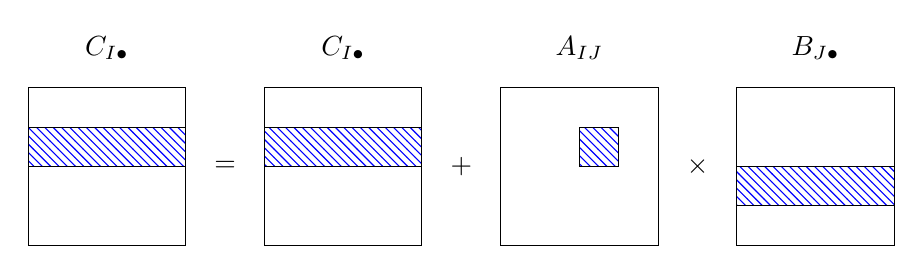
\begin{tikzpicture}
\draw (0, 0) rectangle (2,2); 
\draw (3, 0) rectangle (5,2);
\draw (6, 0) rectangle (8,2); 
\draw (9, 0) rectangle (11,2);

\node (T1) at (1, 2.5) { $C_{I\bullet}$ };
\node (T2) at (4, 2.5) { $C_{I\bullet}$ };
\node (T3) at (7, 2.5) { $A_{IJ}$ };
\node (T4) at (10, 2.5) { $B_{J\bullet}$ };

\node (N1) at (2.5, 1) { $=$ };
\node (N2) at (5.5, 1) { $+$ };
\node (N2) at (8.5, 1) { $\times$ };

\draw[pattern=north west lines, pattern color=blue] (0,1) rectangle (2,1.5);
\draw[pattern=north west lines, pattern color=blue] (3,1) rectangle (5,1.5);
\draw[pattern=north west lines, pattern color=blue] (7,1) rectangle (7.5,1.5);
\draw[pattern=north west lines, pattern color=blue] (9,0.5) rectangle (11,1);
\end{tikzpicture}

\vspace{2cm}

\begin{tikzpicture}
\draw (0,1) rectangle (2,1.5);
\draw (3,1) rectangle (5,1.5);
\draw (7,1) rectangle (7.5,1.5);
\draw (9,0.5) rectangle (11,1);

\node (N1) at (2.5, 1) { $=$ };
\node (N2) at (5.5, 1) { $+$ };
\node (N2) at (8.5, 1) { $\times$ };

\draw[pattern=north west lines, pattern color=blue] (0.5,1.2) rectangle (0.7,1.3);
\draw[pattern=north west lines, pattern color=blue] (3.5,1.2) rectangle (3.7,1.3);
\draw[pattern=north west lines, pattern color=blue] (7,1.2) rectangle (7.5,1.3);
\draw[pattern=north west lines, pattern color=blue] (9.5,0.5) rectangle (9.7,1);

\end{tikzpicture}

\end{document}
